\documentclass[12pt, a4paper]{exam}
\usepackage{graphicx}
\usepackage[margin=0.7in]{geometry}
\usepackage[normalem]{ulem}
\renewcommand\ULthickness{1.0pt}   %%---> For changing thickness of underline
\setlength\ULdepth{1.3ex}%\maxdimen ---> For changing depth of underline
\usepackage{textcomp}
\usepackage{amsmath}
\usepackage{bm}
\usepackage{enumerate}% http://ctan.org/pkg/enumerate
\usepackage{hyperref}
\hypersetup{
    colorlinks=true,
    linkcolor=blue,
    filecolor=magenta,      
    urlcolor=blue,
    }

\urlstyle{same}

% document version
\newcommand{\docver}{\input{version}}

% predefined sets
\newcommand{\bools}{\mathbb{B}}
\newcommand{\nats}{\mathbb{N}}
\newcommand{\ints}{\mathbb{Z}}
\newcommand{\rats}{\mathbb{Q}}
\newcommand{\reals}{\mathbb{R}}
\newcommand{\mts}{\{\}}

% fonts for several objects
\newcommand{\fsys}[1]{\mathsf{#1}}
\newcommand{\fset}[1]{\mathtt{#1}}
\newcommand{\fval}[1]{\mathbf{#1}}
\newcommand{\fsub}[1]{{#1}}
\newcommand{\frlnm}[1]{{\sc #1}}
\newcommand{\extfval}[1]{\overline{\fval{#1}}}
\newcommand{\extfsub}[1]{\overline{\fsub{#1}}}
\newcommand{\fsett}[1]{\mathcal{#1}}
\newcommand{\ff}[1]{\mathit{#1}}
\newcommand{\fp}[1]{\mathit{#1}}
\newcommand{\sort}[2]{{#1}{:}{#2}}

% abbreviations
\newcommand{\fsF}{\fsys{F}}
\newcommand{\DS}{\fsys{DS}}
\newcommand{\DSL}{{\fsys{DS}(\mathcal{L})}}
\newcommand{\LARR}{\mathcal{L}_A}

% Boolean elements
\newcommand{\eF}{\fset{F}}
\newcommand{\eT}{\fset{T}}

% global sets
\newcommand{\vprop}{\fsett{V}}
\newcommand{\prop}{\fsett{T}(\vprop)}
\newcommand{\vars}{\fsett{X}}
\newcommand{\funcs}{\fsett{F}}
\newcommand{\preds}{\fsett{P}}
\newcommand{\lang}{\fsett{L}}
\newcommand{\arity}{\textit{ar}}
\newcommand{\terms}{\fsett{T}_\funcs(\vars)}
\newcommand{\forms}{\fsett{T}_{(\funcs,\preds)}(\vars)}
\newcommand{\srest}[2]{{#2}_{\triangleleft {#1}}}

% logical connectives
\newcommand{\STRUE}{\mathit{true}}
\newcommand{\SFALSE}{\mathit{false}}
\newcommand{\SIFF}{\equiv}
\newcommand{\SXOR}{\not\equiv}
\newcommand{\SOR}{\lor}
\newcommand{\SAND}{\land}
\newcommand{\SNEG}{\neg}
\newcommand{\SIMP}{\rightarrow}
\newcommand{\SCON}{\leftarrow}
\newcommand{\SALL}{\forall}
\newcommand{\SEX}{\exists}

% macros for proposiciones
\newcommand{\TRUE}{\STRUE}
\newcommand{\FALSE}{\SFALSE}
\newcommand{\IFF}[2]{(#1 \SIFF #2)}
\newcommand{\XOR}[2]{(#1 \SXOR #2)}
\newcommand{\OR}[2]{(#1 \SOR #2)}
\newcommand{\AND}[2]{(#1 \SAND #2)}
\newcommand{\NEG}[1]{({\SNEG}#1)}
\newcommand{\IMP}[2]{(#1 \SIMP #2)}
\newcommand{\CON}[2]{(#1 \SCON #2)}
\newcommand{\ALL}[2]{(\SALL{#1}\,{#2})}
\newcommand{\EX}[2]{(\SEX{#1}\,{#2})}

\newcommand{\AIFF}[2]{#1 \SIFF #2}
\newcommand{\AXOR}[2]{#1 \SXOR #2}
\newcommand{\AOR}[2]{#1 \SOR #2}
\newcommand{\AAND}[2]{#1 \SAND #2}
\newcommand{\ANEG}[1]{{\SNEG}#1}
\newcommand{\AIMP}[2]{#1 \SIMP #2}
\newcommand{\ACON}[2]{#1 \SCON #2}
\newcommand{\AALL}[2]{\SALL{#1}\,{#2}}
\newcommand{\AEX}[2]{\SEX{#1}\,{#2}}
\newcommand{\QALL}[3]{(\SALL{#1}\mid {#2}: {#3})}
\newcommand{\QEX}[3]{(\SEX{#1}\mid {#2}: {#3})}
\newcommand{\QALLS}[2]{\left(\SALL{#1}\mid : {#2}\right)}
\newcommand{\QEXS}[2]{\left(\SEX{#1}\mid : {#2}\right)}


% other syntax
\newcommand{\tsub}[3]{#1\!\left[{#2}:={#3}\right]}
\newcommand{\divs}[2]{{#1}\,{\cdot|}\,{#2}}

% environments
\newenvironment{calc}{\begin{array*}}{\end{array*}}
%\newenvironment{calc}{\begin{align*}}{\end{align*}}
\newcommand{\expr}[1]{ & \; {#1} \\}
\newcommand{\exprnnl}[1]{ & {#1}}
\newcommand{\expl}[2]{#1 & \quad \langle \; \textnormal{#2} \;\rangle \\}


\newcommand{\con}[3]{ #1 \overset{#2}{=} #3}
\newcommand{\oexists}[3]{(\exists {#1} \ | \ #2  : \  #3  )}
\newcommand{\oall}[3]{(\forall {#1} \ | \  #2  : \  #3  )}
\newcommand{\hoare}[3]{\{{#1}\} \{{#2}\} \{{#3}\}}
\usepackage{listings}


\begin{document}
	%\thispagestyle{empty}
	\noindent
	\begin{minipage}[l]{0.1\textwidth}
		\noindent
		
\includegraphics[width=1.8\textwidth]{Logosimbolo-uniandes_horizontal.png}
	\end{minipage}
\hfill
\begin{minipage}[c]{0.8\textwidth}
	\begin{center}
		{\large \textbf{Ingeniería de Sistemas y Computación} \par
		\large	Diseño y análisis de algoritmos	\par
		\small  Profesor: Mateo Sanabria Ardila	\par
		\small  Examen 1	\par
		}
	\end{center}
\end{minipage}
\par
\vspace{0.2in}
\noindent
\uline{Fecha de entrega: 01/Marzo 	\hfill  2024-10		\hfill Nota máxima: \textbf{100} }
\par 
\vspace{0.15in}
% {\small \bfseries 	Attempt any five questions }



\begin{questions}
	\pointsdroppedatright
	\question 
    \begin{minipage}{0.7\textwidth}
        Un elemento cumbre en una matriz 2D es un elemento que es  estrictamente mayor que
        todos sus 4-vecinos (izquierda, derecha, arriba, abajo). Dada una matriz de enteros
        positivo, se debe devolver las coordenadas de \textbf{UN} elemento cumbre. Se asume
        que la matriz esta rodeada en su perímetro con el valor -1 en cada celda, como se
        muestra en la imagen. Por ejemplo, para el siguiente caso de prueba se tiene:
        \begin{verbatim}
Input: matrix = [[10,20,15],[21,30,14],[7,16,32]]
Output: [1,1]
Explanation: 30 y 32 som ambos elementos cumbre entonces [1,1] y [2,2] son 
respuesta validas.
        \end{verbatim}
    \end{minipage}%
    \hspace{1em}% Adjust the space between the minipages
    \begin{minipage}{0.2\textwidth}
        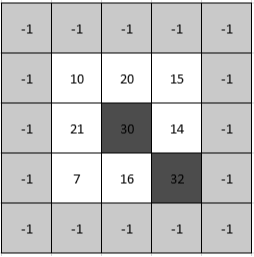
\includegraphics[width=\linewidth]{example-modified.png}
        \label{fig:img1}
    \end{minipage}

    La función \verb|findPeakGrid| implementa un algoritmo en Python que soluciona el
    problema:
\begin{lstlisting}[language=Python]
def findPeakGrid(matrix: list[list[int]]):
	return _find_peak_grid(matrix, 0, len(matrix[0]) - 1)

def _find_peak_grid(matrix: list[list[int]], left: int, right: int):
	mid = left + (right - left) // 2
	max_row = 0
	for row in range(len(matrix)):
		if matrix[row][mid] > matrix[max_row][mid]:
			max_row = row

	left_is_big = mid - 1 >= left 
        and matrix[max_row][mid - 1] > matrix[max_row][mid]
	right_is_big = mid + 1 <= right 
        and matrix[max_row][mid + 1] > matrix[max_row][mid]

	# compare mid to left and right
	if not left_is_big and not right_is_big: 
        # found peak in the middle
		return [max_row, mid]
	elif left_is_big:  
        # peak on the left
		return _find_peak_grid(matrix, left, mid)
	else: 
        # peak on the right
		return _find_peak_grid(matrix, mid + 1, right)

\end{lstlisting}
    \begin{parts}
        \part[]  \textbf{(10pts)} Explique la idea de la solución del algoritmo, es decir
        por que el algoritmo sirve para dar solución al problema, \textbf{NO HAGA
        REFERENCIA A CÓDIGO}. El algoritmo utiliza una estrategia de D\&C?

        \part[]  \textbf{(5pts)} Proponga la función $T(n)$ para \verb|findPeakGrid|. 

        \part[]  \textbf{(30pts)} Resuelva la ecuación de recurrencia del punto anterior.
        Si lo necesita, recuerde que la solución para $T(n) = T(n-1) + m$ es $T(n) =
        n*m$.

        \part[]  \textbf{(5pts)} Basado en lo anterior, cual es la complejidad temporal
        de \verb||findPeakGrid?
    \end{parts}
	\question 
    Dadas dos strings (w1,w2) se quiere conocer cual es la longitud de la subsecuencia
    común mas larga entre w1 y w2. Por ejemplo, si w1=`ABC' y w2=`MATEOBASIC' la respuesta
    debería ser 3. 
    \begin{parts}

        \part[] \textbf{(10pts)} Identifique cuales pueden ser los subproblem repetidos
        para este problema, explique que estructura de datos le puede ayudar a no repetir
        problemas. De un ejemplo, expliquelo y justifique porque esa forma de guardar
        subproblemas puede ayudar a solucionar el problema.

        \part[] \textbf{(30pts)} Proponga un algoritmo \verb|Python,Java,...| (\textbf{No
        es valido respuesta es `palabras'}) basada en programación  dinámica que solución
        el problema. Complejidad esperada $\mathcal{O}(|w1||w2|)$, el punto no es valido 
        si no es alcanza esta complejidad.
        
        \part[] \textbf{(5pts)} Explique cual es la complejidad temporal de la solución
        del punto anterior.

        \part[] \textbf{(5pts)} La solución que propuso es Top-Down (TD) o Button-Up (BU)?
        Por que? Si su solución es TD que ventajas tiene contra una solución BU? Si su
        solución es BU que ventajas tiene contra una solución TD? 

    \end{parts}
\end{questions}

\end{document}